\chapter{Introduction}

La transition énergétique engagée en France et en Europe s’accompagne d’une montée en puissance
rapide des énergies renouvelables intermittentes, en particulier de la production photovoltaïque.
Longtemps marginale dans le mix électrique, cette filière occupe désormais une place croissante et sa
trajectoire de développement reste fortement orientée à la hausse dans les prochaines années :

\begin{figure}[htbp]
    \centering
    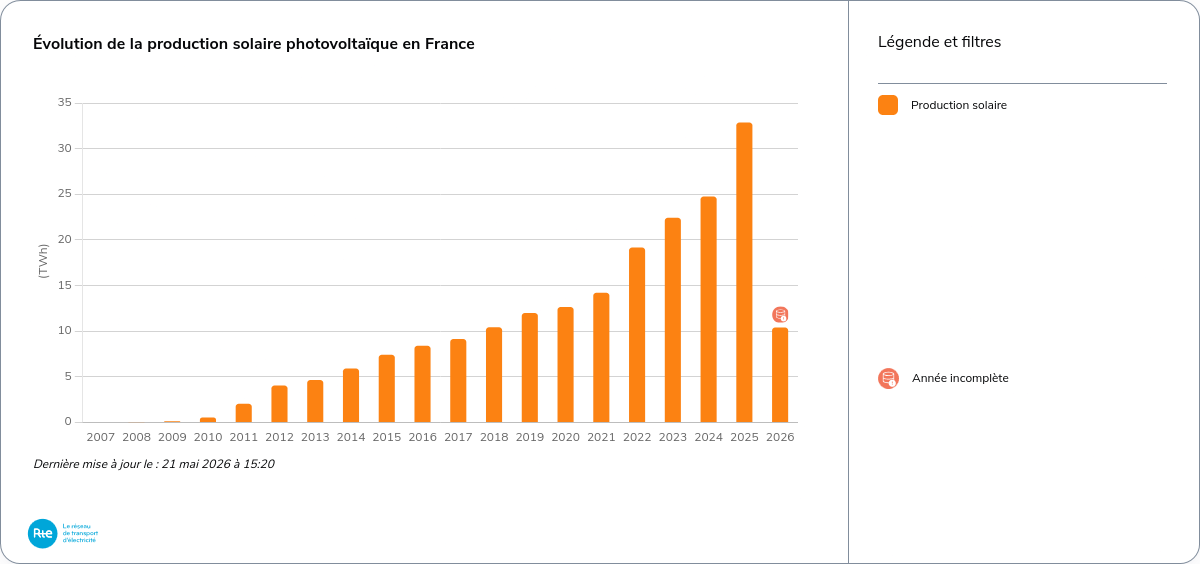
\includegraphics[width=0.7\textwidth]{img/evol_prod_fr.png}
    \caption{Évolution de la production solaire photovoltaïque en France.}
    \label{fig:evolFR}
\end{figure}

Cette figure illustre la croissance soutenue de la production photovoltaïque en France au cours des
dernières années. Cette augmentation rapide contribue à renforcer le rôle du solaire dans le mix
électrique, tout en accentuant les enjeux liés à la variabilité de la production et à son intégration dans le
système électrique. Source : RTE éCO2mix.

Cette évolution constitue un levier majeur de décarbonation du système énergétique, mais introduit
également une dépendance accrue aux conditions météorologiques, qui influencent directement la
disponibilité de la ressource solaire et donc la production effective d’électricité.

Cette transformation impacte particulièrement les réseaux de distribution, qui concentrent une part
importante des installations photovoltaïques décentralisées. Historiquement conçus pour des flux
essentiellement descendants, depuis des moyens de production centralisés vers les consommateurs,
ces réseaux doivent désormais gérer des injections locales variables, parfois importantes et difficilement
pilotables. Pour les gestionnaires de réseaux de distribution, cette évolution introduit de nouvelles
contraintes opérationnelles : risques de surtension, congestions temporaires, sollicitations accrues des
mécanismes de flexibilité, ou encore limitations ponctuelles de production (écrêtement). L’augmentation
continue de la puissance photovoltaïque installée accroît mécaniquement l’exposition à ces situations,
avec pour conséquence potentielle une part croissante d’énergie renouvelable produite mais non
valorisée faute de capacité d’absorption ou d’anticipation suffisante.

Si la prévision de production photovoltaïque fait déjà l’objet de nombreux travaux, notamment à horizon
day-ahead ou intra-journalier, ces approches visent principalement à estimer des niveaux moyens de
production. Or, pour certaines problématiques opérationnelles, les fluctuations rapides de production à
court terme, provoquées par les dynamiques nuageuses, les conditions atmosphériques ou les
variations rapides d’irradiance, constituent un enjeu complémentaire important. Dans ce contexte, le
projet s’est orienté vers une démarche visant à mieux comprendre les mécanismes physiques qui
gouvernent la variabilité photovoltaïque, à structurer un jeu de données enrichi combinant production
observée et variables exogènes explicatives, puis à explorer des approches de modélisation prédictive
adaptées à cette problématique. La richesse et la diversité des facteurs environnementaux susceptibles
d’influencer la production photovoltaïque rendent cette problématique particulièrement adaptée aux
approches de machine learning, capables d’exploiter simultanément de multiples variables explicatives,
de capturer des relations non linéaires complexes et d’aider à identifier les facteurs les plus
déterminants dans la dynamique observée. Cette orientation répondait également à une motivation
pédagogique forte de l’équipe projet, consistant à articuler compréhension physique des phénomènes
énergétiques et mise en œuvre de méthodes avancées de data science.

\section{Objectifs}

Réalisé dans le cadre du cursus \textbf{Data Scientist}, ce projet avait pour objectif de mettre en œuvre, sur une
problématique réelle liée à la transition énergétique, les principales compétences acquises au cours de
la formation : collecte et préparation de données, analyse exploratoire, feature engineering, modélisation
prédictive, évaluation de modèles et interprétation des résultats.

Le cas d’étude retenu portait sur la variabilité de court terme de la production photovoltaïque,
problématique particulièrement intéressante d’un point de vue data science en raison de la multiplicité
des facteurs explicatifs potentiels, de leur forte composante exogène et de la complexité des relations
non linéaires entre environnement physique et production observée.

L’ambition du projet était d’évaluer dans quelle mesure des approches de machine learning pouvaient
contribuer à mieux comprendre et modéliser cette dynamique, en exploitant simultanément un ensemble
riche de variables explicatives issues de sources hétérogènes (production observée, météorologie,
paramètres atmosphériques et données astronomiques).

Plus concrètement, les objectifs poursuivis étaient les suivants :

\begin{itemize}
\item ​Construire un pipeline de collecte et de préparation de données multi-sources cohérent et exploitable
pour un cas d’usage de modélisation ;

\item Explorer les mécanismes physiques influençant la production photovoltaïque et identifier les
variables explicatives pertinentes ;

\item Concevoir des variables dérivées (feature engineering) adaptées à la modélisation de la variabilité de
court terme ;

\item Formuler le problème sous l’angle d’une tâche de machine learning supervisé appliquée aux séries
temporelles ;

\item Expérimenter et comparer différentes approches de modélisation prédictive ;

\item Analyser les performances obtenues ainsi que la contribution relative des différentes variables
explicatives.
\end{itemize}

\clearpage

\section{Equipe}

L’équipe projet réunissait des profils complémentaires, combinant expertise métier, compétences
quantitatives et intérêt pour les approches datascience appliquées à des problématiques complexes.

\textbf{Moustafa Ibrahim} apportait une sensibilité forte aux aspects quantitatifs, mathématiques et à la
modélisation. Son approche a été particulièrement utile pour la formalisation du problème, l’analyse des
dynamiques temporelles et l’évaluation des approches prédictives testées dans le cadre du projet.

\textbf{Christophe Crestey} apportait une expertise métier liée aux systèmes électriques et aux problématiques
opérationnelles des réseaux de distribution, acquise au travers d’une expérience professionnelle dans le
secteur de l’énergie. Cette connaissance a contribué au cadrage du sujet, ainsi qu’à l’interprétation
métier des résultats obtenus. Le projet constituait également pour lui une opportunité d’approfondir
l’usage des techniques de machine learning appliquées au domaine de la data.

\textbf{Mathilde Blanchard} disposait d’un profil scientifique orienté vers l’analyse de données et les approches
d’intelligence artificielle. Son expertise a contribué à la structuration méthodologique du projet, à la
rigueur des analyses et à l’exploration des approches de modélisation, avec une appétence particulière
pour les mécanismes d’apprentissage automatique et leur mise en œuvre technique.

Dans l’ensemble, si l’expertise métier énergétique était plus marquée chez certains membres de
l’équipe, le projet s’inscrivait précisément dans une logique d’apprentissage, permettant de croiser
compréhension physique des phénomènes énergétiques et montée en compétence collective sur les
méthodes de data science.

\section{Interactions avec des experts métier}

Le projet n’a pas donné lieu à un dispositif formel d’entretiens structurés avec des experts externes
dédiés à la problématique. En revanche, le cadrage du sujet s’est appuyé sur une connaissance métier
préexistante des problématiques de réseaux électriques de distribution, notamment liées à l’intégration
croissante des productions renouvelables décentralisées.

L’expérience professionnelle de certains membres de l’équipe dans le secteur de l’énergie a permis
d’ancrer le projet dans des problématiques opérationnelles concrètes, telles que la gestion des
contraintes réseau, l’impact des fluctuations de production photovoltaïque sur l’exploitation, ou encore
les enjeux d’anticipation liés à l’intermittence des énergies renouvelables.

Au-delà de cette expertise embarquée, des échanges informels avec l’environnement professionnel ont
contribué à conforter la pertinence du sujet, notamment sur l’intérêt croissant porté aux problématiques
de prévision, de flexibilité et d’intégration des ENR dans les infrastructures électriques.

\clearpage

\section{Projets similaires, environnement métier}

Des problématiques proches existent déjà dans l’écosystème énergétique, notamment autour de la
prévision de production des énergies renouvelables, en particulier à des horizons day-ahead ou
intra-journaliers. Ces approches visent principalement à anticiper les niveaux de production agrégés
nécessaires à l’équilibrage du système électrique, à l’optimisation des mécanismes de marché ou à
l’exploitation opérationnelle des infrastructures électriques.

Le projet a également bénéficié d’une exploration approfondie de l’écosystème \textbf{open data énergétique},
qui constitue aujourd’hui une source particulièrement riche d’inspiration méthodologique et de données.
Les plateformes ouvertes telles que \textbf{RTE éCO2mix}, l’\textbf{Agence ODRE} (Open Data Réseaux Énergies),
\textbf{ENTSO-E}, ou encore différentes sources météorologiques ouvertes, illustrent la dynamique croissante
de mise à disposition de données énergétiques et environnementales exploitables dans des approches
de data science. Cette ouverture a fortement contribué au cadrage du projet, tant dans le choix des
variables étudiées que dans la structuration du pipeline de collecte et d’enrichissement des données.

Dans l’environnement professionnel de certains membres de l’équipe, les enjeux liés à l’intégration des
productions renouvelables distribuées, à l’anticipation des contraintes réseau et à l’exploitation de
données énergétiques sont des sujets bien identifiés. Toutefois, les approches observées sont
généralement orientées vers des usages opérationnels ciblés de prévision ou de supervision, plutôt que
vers une exploration explicite de la variabilité de court terme et de ses facteurs explicatifs physiques.

Le projet s’inscrit ainsi davantage comme une \textbf{démarche exploratoire de data science appliquée},
inspirée par les problématiques réelles du secteur énergétique et rendue possible par la richesse
croissante de l’open data, plutôt que comme la reproduction directe d’un dispositif existant.
